% Author: Hadrian Lau
% Website: https://www.hadrian.cc
% License: LaTeX Project Public License (LPPL)

\documentclass[a4paper,12pt]{article}

% Packages
\usepackage[utf8]{inputenc}
\usepackage[english]{babel}
\usepackage{amsmath, amsthm, amssymb, amsfonts}
\usepackage{graphicx}
\usepackage{setspace}
\usepackage{geometry}
\usepackage{float}
\usepackage{framed}
\usepackage[dvipsnames,svgnames]{xcolor}
\usepackage[most]{tcolorbox}
\usepackage{thmtools}
\usepackage{apacite}
\usepackage{indentfirst}
\usepackage{chemfig}
\usepackage{pgfplots}
\usepackage[version=4,arrows=pgf-filled,mathfontname=mathsf]{mhchem}
\usepackage{fancyhdr}
\usepackage{titlesec}
\usepackage{xpatch}
\usepackage{blindtext}
\usepackage{hyperref}
\usepackage{empheq}

% Settings
\pgfplotsset{width=15cm,compat=1.18}
\geometry{margin=1in}
\setstretch{1.5}
\newcommand{\HRule}[1]{\rule{\linewidth}{#1}}

% Box equations
\makeatletter
\newcommand{\colorboxed}[1]{\fcolorbox{DarkSeaGreen}{DarkSeaGreen!20}{\m@th$\displaystyle#1$}}
\xpatchcmd{\@Aboxed}{\boxed}{\colorboxed}{}{}
\makeatother

% Note sections
\makeatletter
\NewDocumentCommand{\mynote}{+O{}+m}{%
	\begingroup
	\tcbset{%
		noteshift/.store in=\mynote@shift,
		noteshift=1.5cm
	}
	\begin{tcolorbox}[nobeforeafter,
		enhanced,
		sharp corners,
		toprule=1pt,
		bottomrule=1pt,
		leftrule=0pt,
		rightrule=0pt,
		colback=DarkSeaGreen!20,
		#1,
		left skip=\mynote@shift,
		right skip=\mynote@shift,
		overlay={\node[right] (mynotenode) at ([xshift=-\mynote@shift]frame.west) {\textbf{Note:}} ;},
		]
		#2
	\end{tcolorbox}
	\endgroup
}
\makeatother

% Header and Footer
\pagestyle{fancy}
\fancyhf{}
\fancyhead[L]{Pendulum and Projectile Motion} % HERE
\fancyhead[R]{\thepage}

% Document
\begin{document}
	
	% Front page
	\title{ \normalsize \textsc{}
		\\ [2.0cm]
		\HRule{1.5pt} \\
		\LARGE \textbf{
			\uppercase{Pendulum and Projectile Motion} % HERE
			\HRule{2.0pt} \\ [0.6cm] 
			\LARGE{SPH3U Unit 1 Lab} % HERE
			\vfill
		}
	}
	\date{}
	\author{
		\textbf{Hadrian Lau Yiu Hei} \\ 
		DSC International School \\
		26th September, 2025\\ %HERE
		\href{https://hadrian.cc}{{\color{blue}\underline{\LaTeX\, document code}}}
	}
	\maketitle
	\thispagestyle{empty}
	
	\newpage

	% Table of content
	\setcounter{page}{1}
	\tableofcontents
	\newpage
	
	% Content
	\section{Pendulum Motion}
	The purpose of the pendulum motion lab is to determine the acceleration due to gravity. A pendulum with a string length of 0.33m, attached with a 1.5cm in diameter steel ball, is dropped from a $5^\circ$ from the right without external forces. We recorded the time it takes for 10 oscillations for a total of 3 times for maximum accuracy. 
	
	\subsection{Raw data}
	Length of pendulum wire: $L=33\text{cm}=0.33\text{m}$\\
	Initial angular displacement: $\theta=5^\circ$ to the right\\
	Mass of pendulum bob: $M=?$\\
	Bob diameter: $d=1.5\text{cm}=0.015\text{m}$
	
	\subsection{Actual time trials}
	We did a total of 3 trials, each measuring the time for 10 pendulum oscillations to occur:
	\begin{align*}
		t_1&=11.66\text{s}\\
		t_2&=11.85\text{s}\\
		t_3&=11.65\text{s}
	\end{align*}\\
	The average actual time for 10 oscillations is:
	\begin{align*}
		t_{10avg}&=\frac{11.66\text{s}+11.85\text{s}+11.65\text{s}}{3}\\
		&=\frac{35.16\text{s}}{3} \\
		t_{10avg}&=11.72\text{s}\\
	\end{align*}
	
	So, the average actual time for 1 oscillations is:
	\begin{align*}
		t_{avg}&=\frac{11.72\text{s}}{10}\\
		\Aboxed{t_{avg}&=1.172\text{s}}
	\end{align*}
	
	\subsection{Theoretical time}
	We can calculate the theoretical time for each oscillation under perfect conditions using the simple harmonic motion equation:
	\begin{align*}
		t_{the}&=2\pi\times\sqrt{\frac{L}{g}}\\
		&=2\pi\times\sqrt{\frac{0.33\text{m}}{9.81\text{m}/\text{s}^2}}  \\
		&=2\pi\times\sqrt{0.034\text{s}^2}\\
		&=2\pi\times 0.183\text{s} \\
		\Aboxed{t_{the}&=1.15\text{s}}
	\end{align*} 
	
	\subsection{Error sources}
	Our actual time measurements are quite accurate. There is a very small difference between our actual time and the theoretical time:
	\begin{align*}
		\Delta&=1.172\text{s}-1.15\text{s} \\
		&=0.022\text{s}\\
	\end{align*}
	
	This marginal time difference can be caused by errors like:
	\begin{itemize}
		\item Imprecise measurements: EXPLAIN
		\item Gross errors: EXPLAIN
	\end{itemize}
	
	\newpage
	
	\section{Projectile motion}
	The purpose of the projectile motion lab is to determine the properties of a projectile through displacement graphs, velocity graphs, and a variety of data. We placed a steel ball at the top of the ramp, and captured the trajectory of the steel ball using a slow motion camera.
	
	\subsection{Raw data}
	After reviewing the slow motion video, we can compile the following data points:
	\begin{center}
		\begin{tabular}{ |c|c|c| } 
			\hline
			$\vec{\Delta d_x}$ (m [$\rightarrow$]) & $\vec{\Delta d_y}$ (m [$\uparrow$]) & t (s)\\ 
			\hline\hline
			0.000m & 0.158m & 0.000s\\
			\hline 
			0.015m & 0.146m & 0.030s\\ 
			\hline
			0.030m & 0.128m & 0.060s\\
			\hline
			0.045m & 0.105m & 0.090s \\
			\hline
			0.060m & 0.068m & 0.120s\\
			\hline
			0.075m & 0.023m & 0.150s \\
			\hline
			0.083m & 0.000m & 0.165s\\
			\hline
		\end{tabular} 
	\end{center}
	\bigskip
	\mynote{We measured everything using the steel ball's center.}
	\mynote{The steel ball is tracked using a 1.5cm grid plane. These values are obtained by scaling the values obtained on the grid plane.}
	
	\newpage
	
	\subsection{Calculations}
	All calculations are based on the table of values. 
	\subsubsection{Total Displacement (x-axis)}
	The total displacement in the x-axis:
	\begin{align*}
		\vec{\Delta d}_x&=\vec{\Delta d}_{xf}-\vec{\Delta d}_{xi}\\
		&=0.083 \text{m}\;[\rightarrow]-0.0 \text{m}\; [\rightarrow]\\
		\Aboxed{\vec{\Delta d}_x&=0.083\text{m}\; [\rightarrow]}
	\end{align*}
	\subsubsection{Total Displacement (y-axis)}
	The total displacement in the y-axis
	\begin{align*}
		\vec{\Delta d}_y&=\vec{\Delta d}_{yf}-\vec{\Delta d}_{yi}\\
		&=0.0 \text{m}\; [\uparrow]-0.158 \text{m}\; [\uparrow]\\
		&=-0.158\text{m}\; [\uparrow]\\
		\Aboxed{\vec{\Delta d}_y&=0.158\text{m}\; [\downarrow]}
	\end{align*}
	\subsubsection{Initial Velocity \& Final Velocity (x-axis)}
	According to the laws of projectile motion, $\vec{v_{ix}}=\vec{v_{fx}}$.
	\begin{align*}
		\vec{\Delta d}_x&=\frac{\vec{v_{ix}}+\vec{v_{fx}}}{2}\times \Delta t\\
		&=\frac{2\vec{v_x}}{2}\times \Delta t\\
		&=\vec{v_x}\times \Delta t\\
		0.083\text{m}\; [\rightarrow]&=\vec{v_x} \times 0.17\text{s}\\
		\vec{v_x}&=\frac{0.083\text{m}\; [\rightarrow]}{0.17\text{s}}\\
		\vec{v_x}&=0.49\text{m}/\text{s}\;[\rightarrow]\\
		\Aboxed{\vec{v_{ix}}=\vec{v_{fx}}&=0.49\text{m}/\text{s}\;[\rightarrow]}
	\end{align*}
	\subsubsection{Initial Velocity (y-axis)}
	Since we did not push the steel ball downwards, gravity is the only force that affects it. Hence, when the steel ball is slid down from the ramp, then:
	\begin{align*}
		\Aboxed{\vec{v_{iy}}&=0\text{m}/\text{s}\;[\emptyset]}\\
	\end{align*}
	\subsubsection{Final Velocity (y-axis)}
	The final velocity in the y-axis:
	\begin{align*}
		\vec{\Delta d}_y&=\Delta t\left(\vec{v}_{fy}-\frac{1}{2}\vec{a}_y\Delta t\right)\\
		0.158\text{m}\;[\downarrow]&=0.17\text{s}\left(\vec{v}_{fy}-\frac{1}{2}\left(9.81\text{m}/\text{s}^2\;[\downarrow]\right)0.17\text{s}\right)\\
		\frac{0.158\text{m}\;[\downarrow]}{0.17\text{s}}&=\vec{v}_{fy}-\frac{1}{2}\times9.81\text{m}/\text{s}^2\;[\downarrow]\times0.17\text{s}\\
		0.93\text{m}/\text{s}\;[\downarrow]&=\vec{v}_{fy}-0.83\text{m}/\text{s}\;[\downarrow]\\
		\Aboxed{\vec{v}_{fy}&=1.76\text{m}/\text{s}\;[\downarrow]}
	\end{align*}
	\subsubsection{All calculations}
	Here are all the calculated values:
	\begin{align*}
		\vec{\Delta d}_x&=0.083\text{m}\; [\rightarrow]\\
		\vec{\Delta d}_y&=0.158\text{m}\; [\downarrow]\\
		\vec{v_{ix}}&=0.49\text{m}/\text{s}\;[\rightarrow]\\
		\vec{v_{fx}}&=0.49\text{m}/\text{s}\;[\rightarrow]\\
		\vec{v_{iy}}&=0\text{m}/\text{s}\;[\emptyset]\\
		\vec{v_{fy}}&=1.76\text{m}/\text{s}\;[\downarrow]\\
	\end{align*}
	\subsection{Position-Time graph}
	\begin{center}
		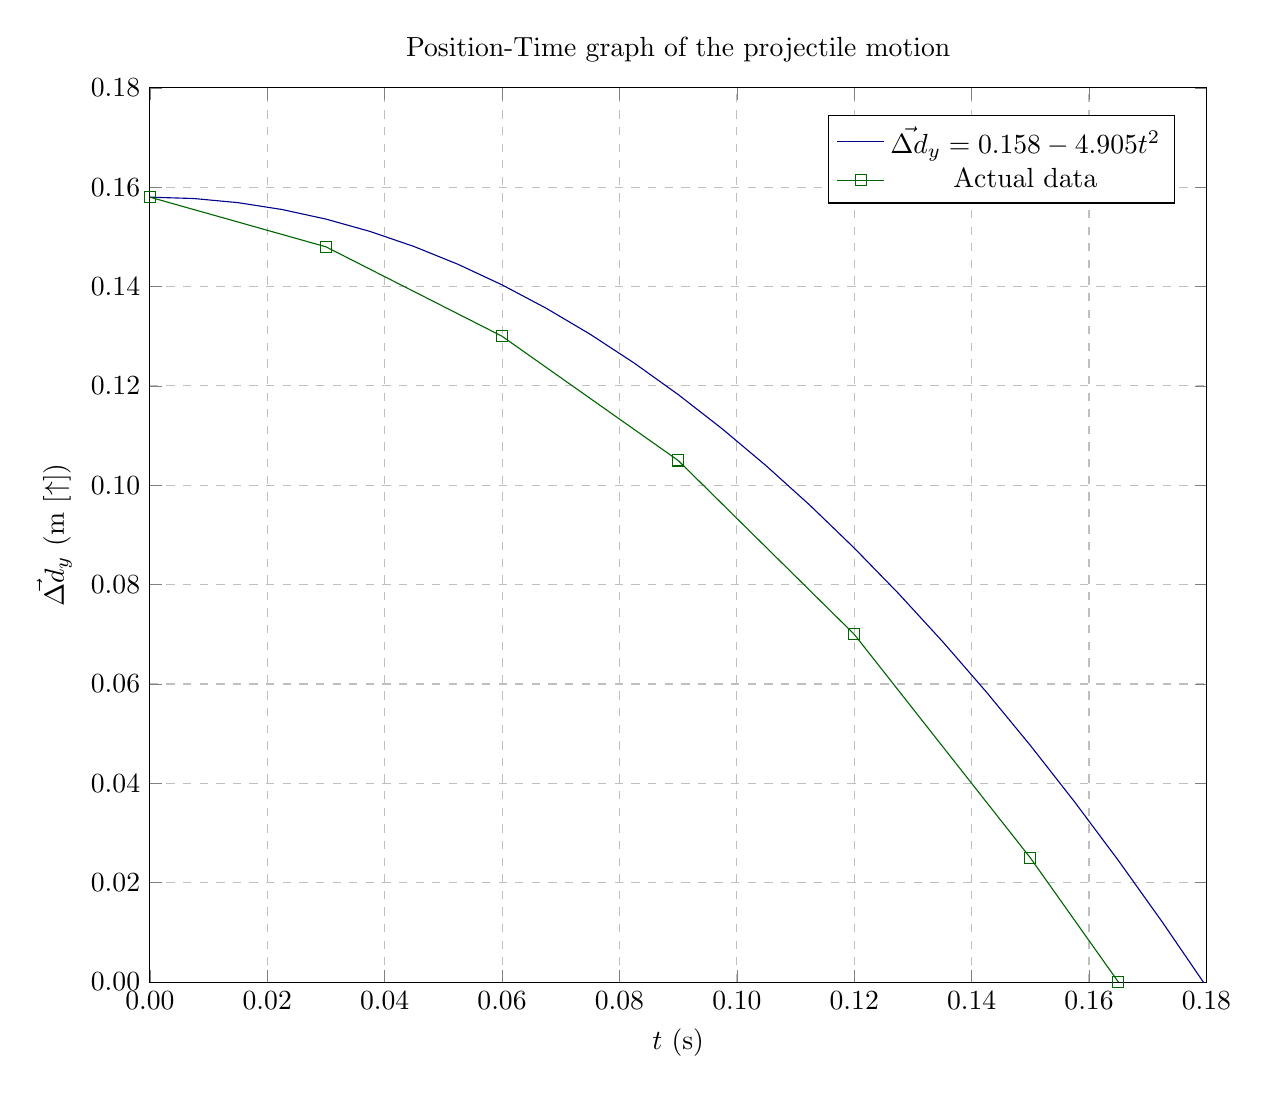
\begin{tikzpicture}
			\begin{axis} [
				title={Position-Time graph of the projectile motion},
				xlabel={$t$ (\text{s})},
				ylabel={$\vec{\Delta d}_y$ (\text{m} [$\uparrow$])},
				xmin=0, xmax=0.18,
				ymin=0, ymax=0.18,
				y tick label style={/pgf/number format/fixed,
					/pgf/number format/fixed zerofill={true}},
				x tick label style={/pgf/number format/fixed,
					/pgf/number format/fixed zerofill={true}},
				xtick distance=0.02,
				ytick distance=0.02,
				ymajorgrids=true,
				xmajorgrids=true,
				legend pos=north east,
				grid style=dashed,
			]	
				\addplot[
					color=DarkBlue,
					domain=0:0.18,
				] {
					0.158-4.905*x*x
				};
				\legend{$\vec{\Delta d}_y=0.158-4.905t^2$, Actual data}
				\addplot[
					color=DarkGreen,
					mark=square,
				] coordinates {
					(0,0.158)(0.03,0.148)(0.06,0.13)(0.09,0.105)(0.12,0.07)(0.15,0.025)(0.165,0)
				};
			\end{axis}
		\end{tikzpicture}
	\end{center}
	\subsection{Velocity-Time graph}
	We calculate the velocity by calculating the slope of each interval in the position time graph:
	\begin{align*}
		m_0&=0\\
		m_1=\frac{y_1-y_0}{x_1-x_0}=\frac{0.146-0.158}{0.03-0}=\frac{-0.012}{0.03}&=-0.4\\
		m_2=\frac{y_2-y_1}{x_2-x_1}=\frac{0.128-0.146}{0.06-0.03}=\frac{-0.018}{0.03}&=-0.6\\
		m_3=\frac{y_3-y_2}{x_3-x_2}=\frac{0.105-0.128}{0.09-0.06}=\frac{-0.023}{0.03}&\approx-0.767\\	m_4=\frac{y_4-y_3}{x_4-x_3}=\frac{0.068-0.105}{0.12-0.09}=\frac{-0.037}{0.03}&\approx-1.233\\
		m_5=\frac{y_5-y_4}{x_5-x_4}=\frac{0.023-0.068}{0.15-0.12}=\frac{-0.045}{0.03}&=-1.5\\
		m_6=\frac{y_6-y_5}{x_6-x_5}=\frac{0-0.023}{0.165-0.15}=\frac{-0.023}{0.015}&\approx-1.533
	\end{align*}
	\begin{center}
		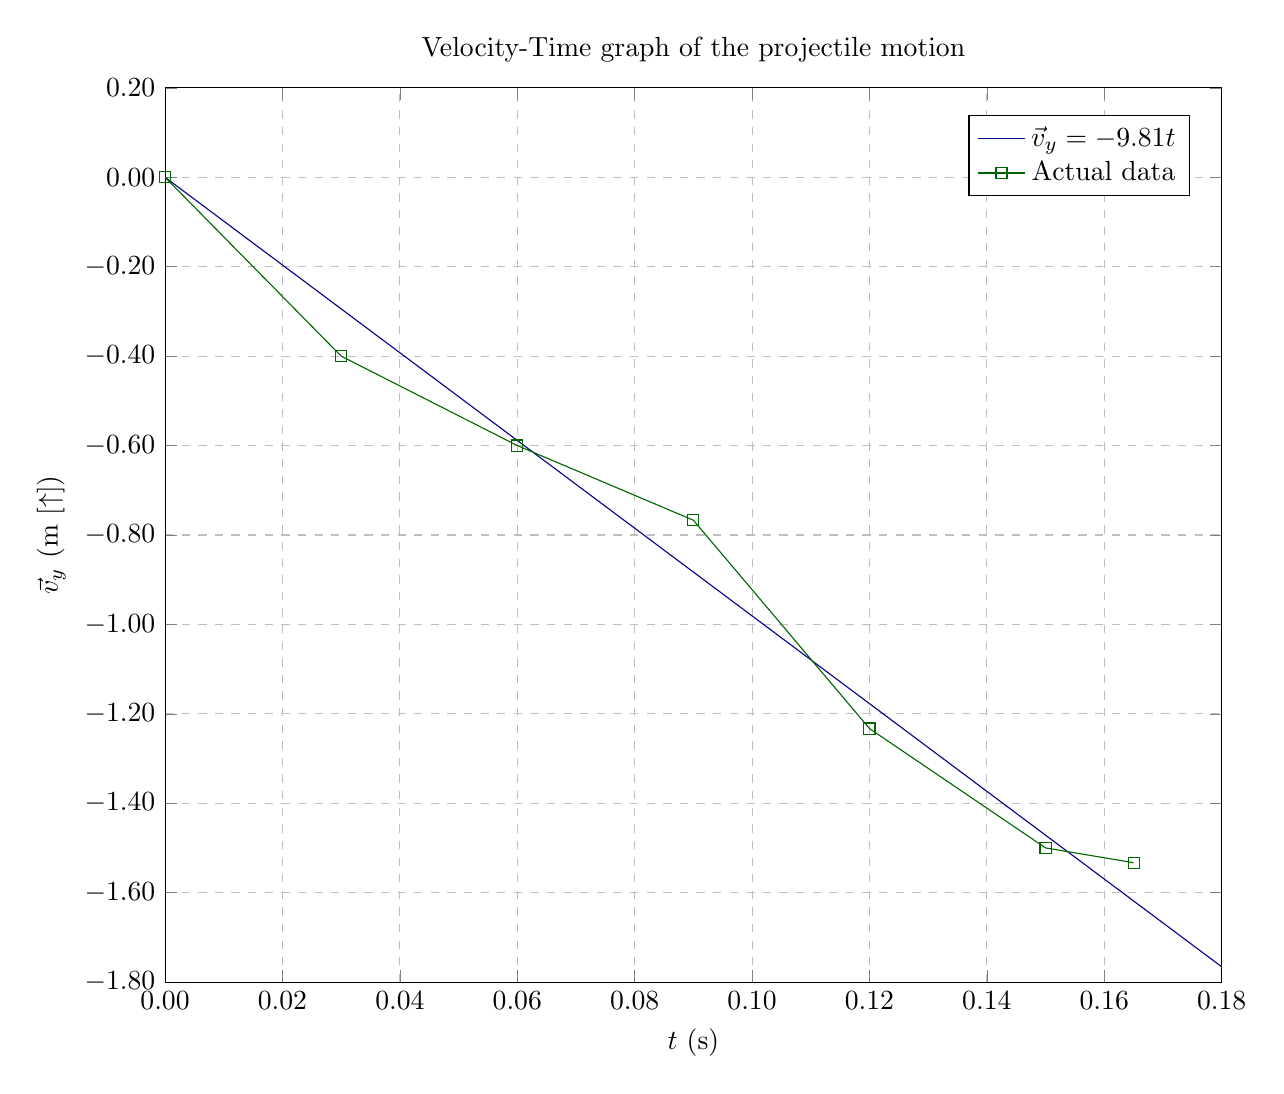
\begin{tikzpicture}
			\begin{axis} [
				title={Velocity-Time graph of the projectile motion},
				xlabel={$t$ (\text{s})},
				ylabel={$\vec{v}_y$ (\text{m} [$\uparrow$])},
				xmin=0, xmax=0.18,
				ymin=-1.8, ymax=0.2,
				y tick label style={/pgf/number format/fixed,
					/pgf/number format/fixed zerofill={true}},
				x tick label style={/pgf/number format/fixed,
					/pgf/number format/fixed zerofill={true}},
				xtick distance=0.02,
				ytick distance=0.2,
				ymajorgrids=true,
				xmajorgrids=true,
				grid style=dashed,
				legend pos=north east,
				]			
				\addplot[
					color=DarkBlue,
					domain=0:0.18,
				] {
					-9.81*x
				};
				\legend{$\vec{v}_y=-9.81t$, Actual data}
				\addplot[
					color=DarkGreen,
					mark=square,
				] coordinates {
					(0,0)(0.03,-0.4)(0.06,-0.6)(0.09,-0.767)(0.12,-1.233)(0.15,-1.5)(0.165,-1.533)
				};
			\end{axis}
		\end{tikzpicture}
	\end{center}
	
	\newpage
	
	\section{Licensing}
	All LaTeX packages are provided by TeX Live under the LaTeX Project Public License (LPPL).\\
	The pgfplots package is licensed under the GNU General Public License (GPL) version 3 or later.\\
	The titlesec package is licensed under the MIT License.\\
	Template created by Hadrian Lau, derived from the HKUST Lab Report Template by Ma Wanqin, distributed under the Creative Commons CC BY 4.0 license.\\
	The LaTeX engine is provided by TeX Live under the LaTeX Project Public License (LPPL).\\
	NixOS Linux Operating System is distributed under the GNU Lesser General Public License (LGPL) version 2.1.\\
	The LaTeX code editor is provided by TeXstudio under the GNU General Public License (GPL) version 2.\\
	The LaTeX typesetting system is distributed under the LaTeX Project Public License (LPPL).\\
	
	%\newpage
	%\bibliographystyle{plain}
	%\bibliography{references}  % Add a .bib file if you have references
	
\end{document}

% All LaTeX packages are provided by TeX Live under the LaTeX Project Public License (LPPL).
% The pgfplots package is licensed under the GNU General Public License (GPL) version 3 or later.
% The titlesec package is licensed under the MIT License.
%
% Template created by Hadrian Lau, derived from the HKUST Lab Report Template by Ma Wanqin, distributed under the Creative Commons CC BY 4.0 license.
%
% The LaTeX engine is provided by TeX Live under the LaTeX Project Public License (LPPL).
% NixOS Linux Operating System is distributed under the GNU Lesser General Public License (LGPL) version 2.1.
% The LaTeX code editor is provided by TeXstudio under the GNU General Public License (GPL) version 2.
% The LaTeX typesetting system is distributed under the LaTeX Project Public License (LPPL).


